%!TEX root = ../var.tex


Теория вероятностей, как и любая современная математическая теория,
начинается с аксиоматических (неопределяемых) понятий. Такими являются
следующие понятия.
\begin{enumerate}
	\item Понятие: \textit{эксперимент = опыт = испытание}. Считается, что все три
слова означают одно и то же, т.е. являются синонимами.
	\item Понятие: \textit{произойти = возникнуть = появиться}.
	\item Понятие: \textit{элементарное событие = элементарный исход = результат
= шанс}.
\end{enumerate}

При этом считается, что в результате опыта происходит одно и только
одно элементарное событие.

\begin{definition}
	Множество всех элементарных событий данного эксперимента называется \textit{пространством элементарных событий}, или часто короче \textit{пространством}.
\end{definition}

Будем обозначать его через $\Omega$. 
Ясно, что пространство элементарных событий не пусто, $\Omega\ne\noo$.

Как множество пространство $\Omega$ может быть либо конечным\footnote{Конечное множество -- множество, количество элементов которого конечно, то есть, существует неотрицательное целое число n, равное количеству элементов этого множества. В противном случае множество
называется бесконечным.}, 
либо счётным\footnote{Cчётное множество есть бесконечное множество, элементы которого можно пронумеровать натуральными числами. Более формально: множество $\Omega$ является счётным, если существует биекция $\Omega\leftrightarrow N$, где $N$ обозначает множество всех натуральных чисел.}, 
либо несчётным множеством\footnote{Множество, не являющееся конечным или счетным, называется несчетным.}.

\begin{definition}
	Конечные и счётные пространства элементарных событий называются \textit{дискретными}.
\end{definition}

\textbf{Примеры}. 
\begin{enumerate}
	\item Эксперимент: подбрасывание монеты. Элементарные события: $o$ -- выпадение орла, $p$ -- выпадение решётки. Пространство $\Omega=\{o,p\}$ является конечным множеством.
	\item Эксперимент: одновременное подбрасывание двух монет одного достоинства. Пространство элементарных событий $\Omega=\{(o,o),(o,p),(p,p)\}$ является конечным множеством.
	\item Эксперимент: подбрасывание одной монеты до выпадения первого орла. Пространство элементарных событий $$\Omega=\{o, po, ppo, pppo, ppppo, pppppo, \ldots\}$$ -- счётное множество.
	\item Эксперимент: на стол $\Omega=I^2=I\times I$ садится мыльный пузырь и лопается, оставляя под собой точку $(x, y)$. Элементарное событие: появление на плоскости точки$ (x, y)$. Пространство элементарных событий $\Omega$ -- несчётное
множество.
\end{enumerate}


\begin{definition}
	\label{def:2.3}
Если пространство $\Omega$ содержит только одно элементарное событие, то эксперимент называется с детерминированным (определённым) исходом; в противном случае эксперимент называется со случайным исходом.
\end{definition}

\begin{definition} 
	\label{def:2.4}
Любое подмножество $A\subset\Omega$ пространства элементарных событий называется случайным событием или просто событием. Считается, что событие $A$ произошло, если произошло любое элементарное событие $\Omega$, содержащееся в $A$, см. рис. \ref{fig1}.
\end{definition}

\begin{definition}
	\label{def:2.5}
	1) Событие $\Omega$ называется \textit{достоверным}.\\
	2) Событие $\noo\subset\Omega$ называется \textit{невозможным}.
\end{definition}

Каждое элементарное событие $\omega\in\Omega$ можно рассматривать как одноэлементное подмножество достоверного события $\Omega$, т.е. $\{\omega\}\subset\Omega$. Для изображения событий можно использовать диаграммы Венна\footnote{Джон Венн (John Venn, 1834 -- 1923), английский логик.}.

Пусть $A$ и $B$ -- события, они показаны на рис. \ref{fig1}.

\begin{figure}[h!]
	\centering
	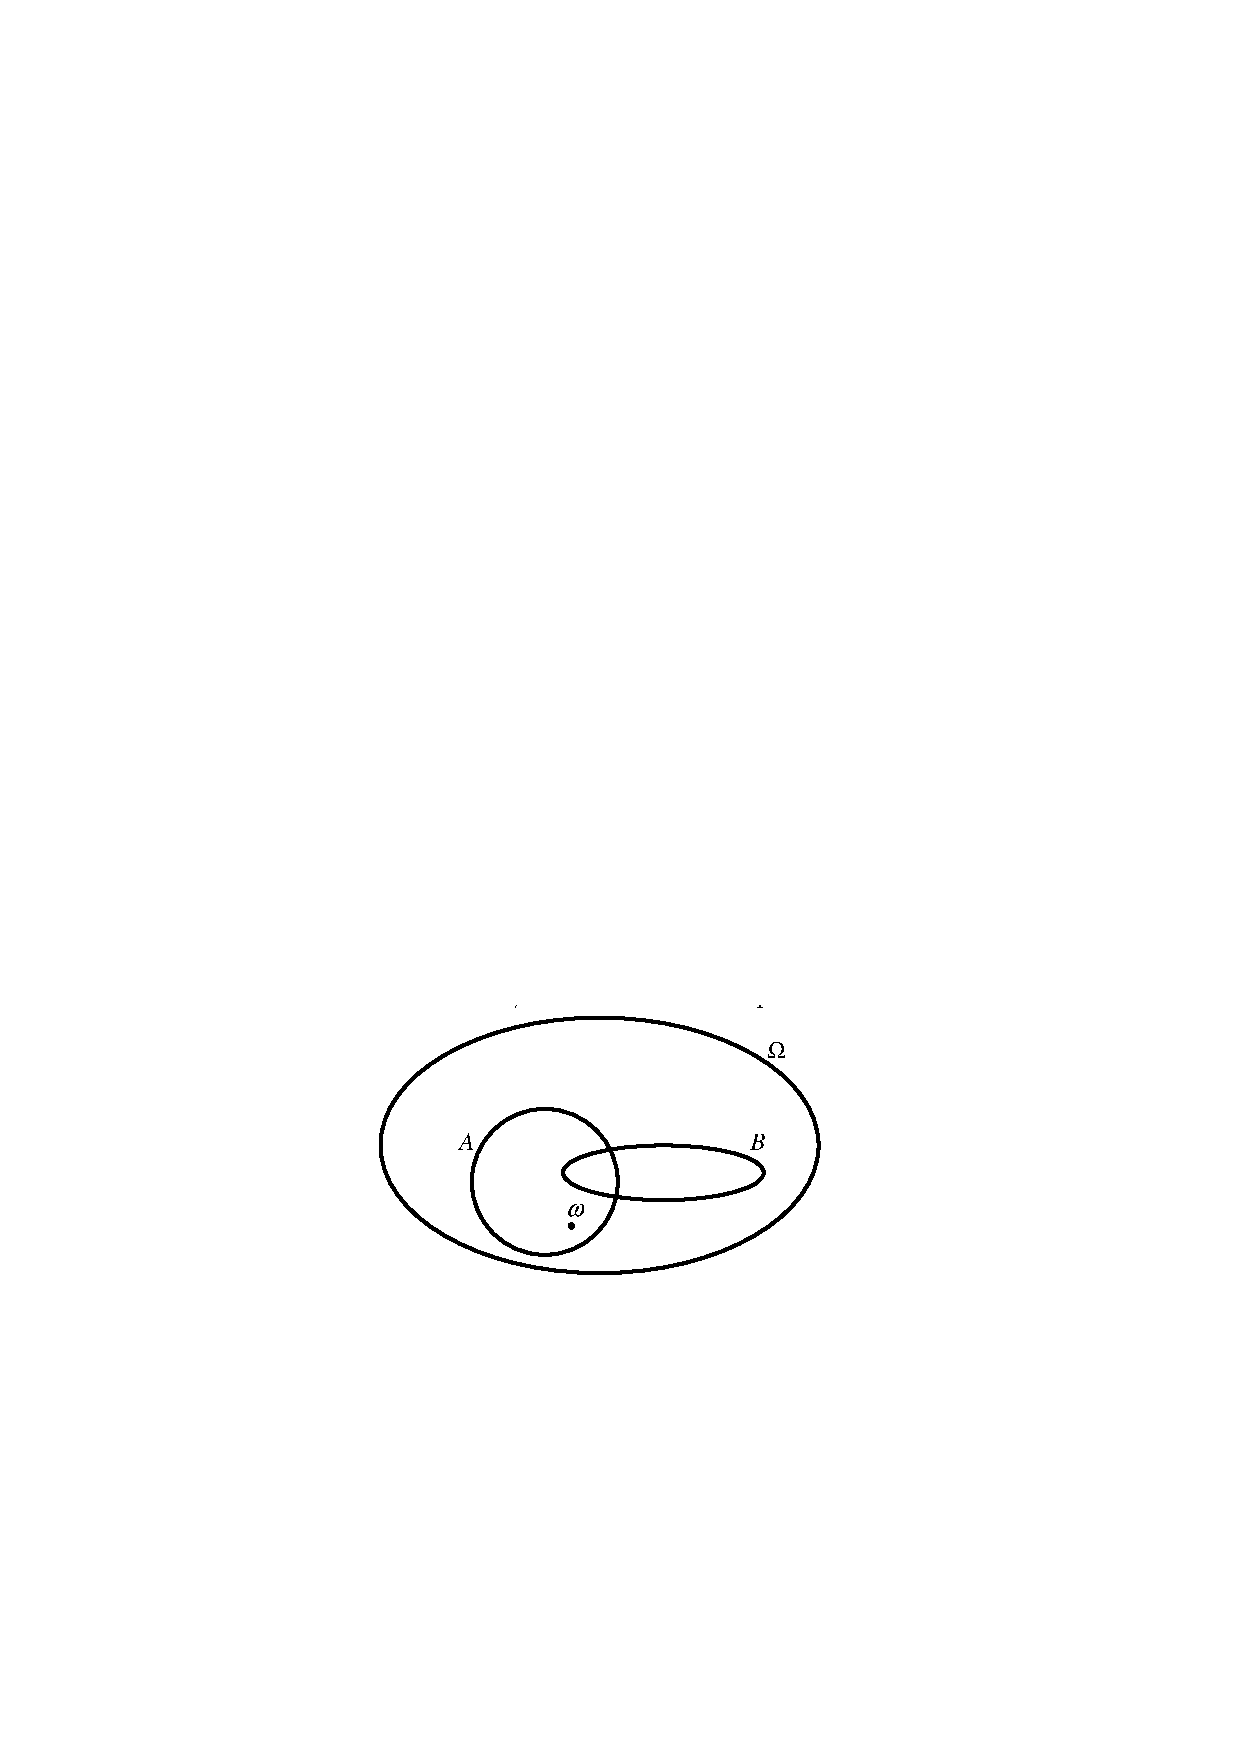
\includegraphics[]{pic/pic1}
	\caption{События в достоверном событии $\Omega$}
	\label{fig1}
\end{figure}

\begin{definition}
	\label{def:2.6}
1) Событие $A \cup B$ называется \textit{объединением} событий и состоит в том, что произошло хотя бы одно из событий $A$ или B.

2) Событие $A\cap B$ называется \textit{пересечением} событий $A$ и $B$ и состоит в
том, что произошли оба события $A$ и B.

3) Событие $A\backslash B$ называется \textit{разностью} событий $A$ и $B$ и состоит в том,
что событие $A$ произошло, а $B$ -- нет.

4) Событие $\overline{A}=\Omega\backslash A$ называется \textit{противоположным событию} $A$ и состоит в том, что событие $A$ не произошло. Ясно, что $A$ = $A$ (событие, противоположное к противоположному, является исходным событием).
Т.к. $\overline{\noo}=\Omega\backslash\noo$ и $\overline{\Omega}=\Omega\backslash\Omega=\noo$, то невозможное событие $\noo$ и
достоверное событие $\Omega$ являются взаимно противоположными (друг другу).

5) Говорят, что событие $A$ \textit{влечёт} событие $B$, и пишут $A\subset B$, если при
наступлении события $A$ происходит и событие $B$.
\end{definition}


\begin{definition}
	\label{def:2.7}
1) События $A$ и $B$ называются \textit{несовместными}, если
$A\cup B$ является невозможным событием, т.е. $A\cup B$ = $\noo$.

2) События $A_1,\cdots,A_n$ называются \textit{попарно несовместными}, если для любых $1\leq i<j\leq n$ события $A_i$ и $A_j$ несовместны.
\end{definition}

\begin{definition}
	\label{def:2.8}
Рассмотрим множество $\mathfrak{A}$, элементами которого являются события пространства $\Omega$ (не обязательно все!). Множество $A$ называется алгеброй событий, если достоверное событие $\Omega$ и любые события $A, B \in A$
удовлетворяют аксиомам:

Акс. $\mathcal{A}1$.$\quad$ $\Omega\in\mathfrak{A}$.

Акс. $\mathcal{A}2$.$\quad$ $A\cup B\in\mathfrak{A}$.

Акс. $\mathcal{A}3$.$\quad$ $A\cap B\in\mathfrak{A}$.

Акс. $\mathcal{A}4$.$\quad$ $A\backslash B\in\mathfrak{A}$.


Из аксиомы $\mathcal{A}1$ следует, что алгебра событий не может быть пустой; она всегда содержит достоверное событие $\Omega$. А т.к. $\Omega \backslash \Omega$ = $\noo$, то из аксиомы $\mathcal{A}4$ следует, что $\noo\in\mathfrak{A}$, т.е. любая алгебра событий $\mathfrak{A}$ содержит вместе с достоверным и невозможное событие.
\end{definition}

\textbf{Примеры}

1) Для любого пространства элементарных событий $\Omega$ набор из двух множеств $\mathfrak{A}_0=\{\noo,\Omega\}$ удовлетворяет аксиомам $\mathcal{A}1$--$\mathcal{A}4$, поэтому $\mathfrak{A}_0=\{\noo,\Omega\}$ является алгеброй событий. Алгебра событий $A_0$ называется тривиальной. Это самая маленькая алгебра событий.

2) В этом примере эксперимент -- подбрасывание игральной кости. 
Пространство элементарных событий есть $\Omega = \{1, 2, 3, 4, 5, 6\}$. 
Пусть событие $A = \{1, 3, 5\}$ -- выпадение нечётного числа очков, а событие $B= \{2, 4, 6\}$ -- выпадение чётного числа очков. 
Множество событий $\mathfrak{A}_1 = \{\noo, \Omega, A, B\}$ удовлетворяет аксиомам $\mathcal{A}1$--$\mathcal{A}4$, поэтому является алгеброй событий.

3) Для любого пространства элементарных событий $\Omega$ множество $\mathfrak{B}(\Omega)$ = множество всех подмножеств $\Omega$ удовлетворяет аксиомам $\mathcal{A}1$--$\mathcal{A}4$, поэтому является алгеброй событий. 
Эта алгебра событий является самой большой на $\Omega$. Для $\Omega= \{1, 2, 3, 4, 5, 6\}$ эта алгебра событий содержит 64 события.

4) Задайте ещё какую-нибудь алгебру событий на $\Omega = \{1, 2, 3, 4, 5, 6\}$.
Сколько различных алгебр событий можно задать на этом пространстве элементарных событий?

\begin{zam}
	\label{zam:2.9}
Из аксиом $\mathcal{A}1$--$\mathcal{A}4$ следует, что если к конечному набору событий из любой алгебры событий применить операции объединения, пересечения и вычитания конечное число раз, то полученное событие тоже содержится в этой алгебре.
\end{zam}

\begin{zam}
	\label{zam:2.10}
Если пространство элементарных событий конечно, $\Omega = \{\omega_1,\omega_2,\ldots,\omega_n\}$, то любая его алгебра событий тоже конечна. 
Это следует из того, что множество $\mathfrak{B}(\Omega)$ всех возможных событий, содержащихся в $\Omega$, тоже конечно и содержит $2^n$ событий.
\end{zam}

\begin{definition}
	\label{def:2.11}
Алгебра событий $\mathfrak{A}$ называется $\sigma$-алгеброй, если для любого счётного набора событий $A_1,A_2,\cdots \in \mathfrak{A}$ выполнена пятая аксиома:

Акс. $\mathcal{A}5$.$\quad$ $\bigcup\limits_{n=1}^\infty A_n \in\mathfrak{A}$.
\end{definition}


\begin{zam}
Из аксиом $\mathcal{A}1$--$\mathcal{A}4$ не следует, что объединение несчётного количества событий является событием из $\sigma$-алгебры. 
Рассмотрение несчётных объединений событий приводит к построению т.н. неизмеримых событий, вероятность наступления которых не существует. 
Первый пример такого неизмеримого события построил Витали\footnote{Джузеппе Витали (Giuseppe Vitali, 26.08.1875 -- 29.02.1932, Italy) -- итальянский математик.}. 
При построении неизмеримого множества Витали используется аксиома теории множеств -- аксиома выбора.
\end{zam}

\textbf{Аксиома выбора.} \textit{Для любого произвольного набора непустых непересекающихся множеств можно составить множество, выбрав в него по одному элементу из каждого множества этого набора.}

\begin{theorem}[Теорема Витали -- построение неизмеримого множества]
\textit{Существуют множества, длина которых не может быть выражена никаким числом.}
\end{theorem}

\begin{proof}
Для доказательства нам понадобятся лишь следующие очевидные свойства длины:

	\begin{itemize}
	\item длина дуги остается неизменной при повороте окружности вокруг
	центра;
	\item длина дуги, которая представляет собой объединение счетного количества попарно непересекающихся дуг, равна сумме длин этих
	дуг.	
	\end{itemize}	

Рассмотрим стандартную (единичного радиуса) окружность $S^1$. Она эквивалентна отрезку $[0, 2\pi)$, т.е. её длина равна $2\pi$. На этой окружности центральный угол в радианах равен длине дуги на которую он опирается.

Для любого рационального числа $\frac{p}{q}$ , где $q\ne 0$, рассмотрим дугу длины $\frac{2\pi p}{q}$.

Если отложить её на окружности $S^1$ последовательно $q$ раз, то полученная дуга замкнётся, т.е. начало 1-ой дуги совпадёт с концом $q$-ой.

Для любого иррационального числа $\alpha$ рассмотрим дугу длины $2\pi\alpha$. Ясно, что если отложить эту дугу $n$ раз на окружности $S^1$, то начало и конец дуги $2\pi\alpha n$ не совпадут ни при каком целом n. Это означает, что множество
\begin{equation*}
	A_0 = \{\ldots, -2\pi\alpha n, \ldots , -4\pi\alpha, -2\pi\alpha, 0, 2\pi\alpha, 4\pi\alpha, \ldots , 2\pi\alpha n, \ldots\}
\end{equation*}

является счётным. Заметим, что для любого целого $n$ поворот на угол $2\pi\alpha n$ переводит множество $A_0$ в себя.
Если взять произвольную точку (угол) $\phi \in [0, 2\pi)$ на окружности, такую чтобы $\phi \notin A_0$ , то множество
\begin{equation*}
	A_\phi = \{\ldots , \phi - 2\pi\alpha n, \ldots , \phi - 4\pi\alpha, \phi - 2\pi\alpha, \phi, \phi + 2\pi\alpha, \phi + 4\pi\alpha, \ldots , \phi + 2\pi\alpha n, \ldots \}
\end{equation*}

тоже является счётным, и для любого целого $n$ поворот множества $A_\phi$ на угол $2\pi n\alpha$ тоже переводит его в себя. 

Заметим, что т.к. $\phi \notin A_0$ , то множества $A_0$
и $A_\phi$ не пересекаются: если бы они имели общую точку, то при $n=\pm1, \pm2, \ldots$ все остальные их точки получились бы прибавлением дуг $2\pi\alpha n$, и тогда бы множества $A_0$ и $A_\phi$ совпадали. 

Заметим, что для любого целого $n$ поворот на
угол $2\pi\alpha n$ переводит множество $A_\phi$ в себя.

Если теперь выбрать угол $\psi \in [0, 2\pi)$, такой чтобы $\psi \notin A_0$ и $\psi \notin A_\phi$ , то множество
\begin{equation*}
	A_\psi = \{\ldots , \psi - 2\pi\alpha n, \ldots , \psi - 4\pi\alpha, \psi - 2\pi\alpha, \psi, \psi + 2\pi\alpha, \psi + 4\pi\alpha, \ldots , \psi + 2\pi\alpha n, \ldots \}
\end{equation*}

тоже является счётным, и для любого целого $n$ поворот множества $A_\psi$ на угол $2\pi\alpha n$ тоже переводит его в себя. Заметим, что т.к. $\psi \notin A_0$ и $\psi \notin A_\phi$, то
множество $A_\psi$ не пересекается ни с $A_0$ и ни с $A_\phi$. 

Заметим, что для любого целого $n$ поворот на угол $2\pi\alpha n$ переводит множество $A_\psi$ в себя.

Процесс построения таких непересекающихся множеств можно продолжить неограниченно
\footnote{
	В математике различают два типа бесконечности: потенциальная и актуальная бесконечности.

	Потенциальная бесконечность означает, что процесс построения какого-либо объекта может быть продолжен неограниченно. В нашем случае процесс построения множеств $A_\phi , A_\xi , A_\psi , \ldots$ может быть продолжен неограниченно (если не принимать во внимание, какое время может быть потрачено на это построение).
	Другой пример потенциальной бесконечности возникает при построении натурального ряда.
	Если мы выпишем все натуральные числа от 1 до $n$, то ничто не мешает нам написать число $n+1$, и т.д.
	Потенциальная бесконечность есть бесконечный процесс построения объектов, у которого нет последнего шага. Например, в доказательстве по методу математической индукции.

	Под актуальной бесконечностью понимается бесконечная совокупность, построение которой завершено, и все ее элементы наличествуют одновременно. Например, мы будем иметь дело с актуальной бесконечностью, если перечислим весь натуральный ряд полностью и имеем его в законченном виде
	$N = \{1, 2, \ldots , n, \ldots \}$. Актуальная бесконечность представляет собой весьма сильную идеализацию. В
	самом деле, она допускает не только возможность построения последующего объекта, если построен
	предыдущий, но и постулирует, что все возможные объекты уже построены и существуют одновременно.
	В нашем случае актуальная бесконечность означает, что процесс построения множеств $A_0, A_\phi, A_\psi , \ldots$
	закончен, и мы имеем это множество множеств $\{A_0, A_\phi, A_\psi , \ldots\}$ налицо.
}, пока не будут исчерпаны (выбраны) все точки окружности $S^1$ . В каждом таком множестве содержится счетное число точек, и все точки в одном множестве получаются друг из друга поворотами на угол $2\pi\alpha$.

Разные множества не пересекаются. Таким образом, окружность $S^1$ является объединением непересекающихся множеств $A_0, A_\phi, A_\psi , \ldots $ т.е.
\begin{equation*}
	S^1=\bigcup\limits_{\lambda\in\{0,\phi,\psi,\ldots\}}A_\lambda
\end{equation*}

Объединение счётного набора счётных множеств есть счётное множество.
А т.к. окружность $S^1$ состоит из несчетного множества точек, то набор построенных множеств $A_0, A_\phi, A_\psi , \ldots $ является несчётным. Другими словами множество индексов $\{0, \phi, \psi, \ldots ,\}$ -- несчётное.

Выберем из каждого множества $A_0, A_\phi, A_\psi , \ldots $ ровно по одной точке и по аксиоме выбора составим из этих точек множество $B_0$. 

Построенное множество $B_0$ называется \textit{множеством Витали}. Для каждого $n=\pm1, \pm2, \ldots$ обозначим через $B_n$ множество, которое получается в результате поворота множества $B_0$ на угол $2\pi n\alpha$. 

Ясно, что все множества $B_n$ , $n\in \mathbb{Z}$, имеют одну и ту же длину. Т.к. все точки множества $A_\lambda$ , где $\lambda \in \{0, \phi, \psi, \ldots\}$, можно получить, поворачивая одну из них на углы $2\pi n\alpha$, и т.к. в множестве $B_0$ собраны по одной точке из каждого множества $A_\lambda$ , то объединение всех $B_n$ составляет окружность $S^1$ , т.е.
\begin{equation*}
	S^1=\bigcup\limits_{n=-\infty}^{\infty}B_n
\end{equation*}

Оставшуюся часть доказательства проведём методом от противного. Предположим, что длина множества Витали $B_0$ существует, и обозначим её через $\mu(B_0)$. Тогда все множества $B_n$ имеют одну и ту же длину, т.к. получены из $B_0$ поворотом на угол кратный $2\pi\alpha$. Т.к. множества $B_n$ не пересекаются, то сумма их длин равна длине окружности $S^1$ . Поэтому

\begin{gather*}
	2\pi=\mu(S^1)=\mu\left(\bigcup\limits_{n=-\infty}^{\infty}B_n\right)=\sum\limits_{n=-\infty}^{\infty}\mu(B_n)=
	\sum\limits_{n=-\infty}^{\infty}\mu(B_0)=\\
	=
	\left\{
		\begin{aligned}
			\infty, \text{если } \mu(B_0)>0\\
			0, \text{если } \mu(B_0)=0
		\end{aligned}
	\right.
\end{gather*}

Полученное противоречие означает, что длины у множества Витали $B_0$ нет вообще никакой (ни нулевой, ни конечной, ни бесконечной). Такие множества и соответствующие им события называются \textit{неизмеримыми}.
\end{proof}

\begin{zam}
1) В предыдущем примере было доказано существование неизмеримого множества (множества Витали) и предъявлена конструкция его построения. Меняя иррациональное число $\alpha$, можно получить несчётное количество неизмеримых множеств на окружности $S^1 = [0, 2\pi)$. 

Если аксиому выбора не признавать, то неизвестно можно ли вообще построить неизмеримые множества. Можно доказать, что аксиома $\mathcal{A}5$ не допускает появление неизмеримых событий.

2) Если $\Omega$ -- несчётное множество (отрезок, площадка, объёмное тело), то множество P($\Omega$) всех подмножеств множества $\Omega$ не является $\sigma$-алгеброй, потому что оно содержит неизмеримые события.
\end{zam}

\begin{zam}
Все конечные и счётные алгебры событий являются $\sigma$-алгебрами.
\end{zam}

\begin{lemma}\label{lemmde}
Если ${A_1 , A_2 , \ldots }$ есть счётный набор событий из $\sigma$-алгебры $A$, то $\bigcap\limits_{n=1}^\infty A_n\in\mathfrak{A}$
\end{lemma}

\begin{proof}
Пусть $A1 , A2 , \ldots \in \mathfrak{A}$, Тогда из аксиомы $\mathcal{A}4$ следует, что
	\begin{equation*}
		\overline{A}_1,\overline{A}_2, \ldots \in \mathfrak{A},
	\end{equation*}
а из аксиомы $\mathcal{A}5$ следует, что
	\begin{equation*}
		\bigcup\limits_{n=1}^\infty \overline{A}_n\in\mathfrak{A}.
	\end{equation*} 
Тогда по аксиоме 4 дополнение к этому множеству тоже принадлежит $\mathfrak{A}$, т.е. 
	\begin{equation*}
		\overline{\bigcup\limits_{n=1}^\infty \overline{A}_n}\in\mathfrak{A}
	\end{equation*}
по формулам двойственности де Моргана
	\begin{equation*}
		\overline{\bigcup\limits_{n=1}^\infty \overline{A}_n}=\bigcap\limits_{n=1}^\infty {A}_n,
	\end{equation*} 
поэтому
	\begin{equation*}
		\bigcap\limits_{n=1}^\infty {A}_n\in\mathfrak{A}
	\end{equation*}

\end{proof}

\begin{consq}
	Лемма \ref{lemmde} и аксиома $\mathcal{A}5$ эквивалентны.
\end{consq}